\documentclass[a4paper, 12pt]{report}
\usepackage{setting}

\setstretch{1.2}

\title{TFG Jaume}
\author{Jaume Casals Vilaplana}
\date{\today}

\begin{document}

\pagenumbering{gobble} % Avoid page numbering
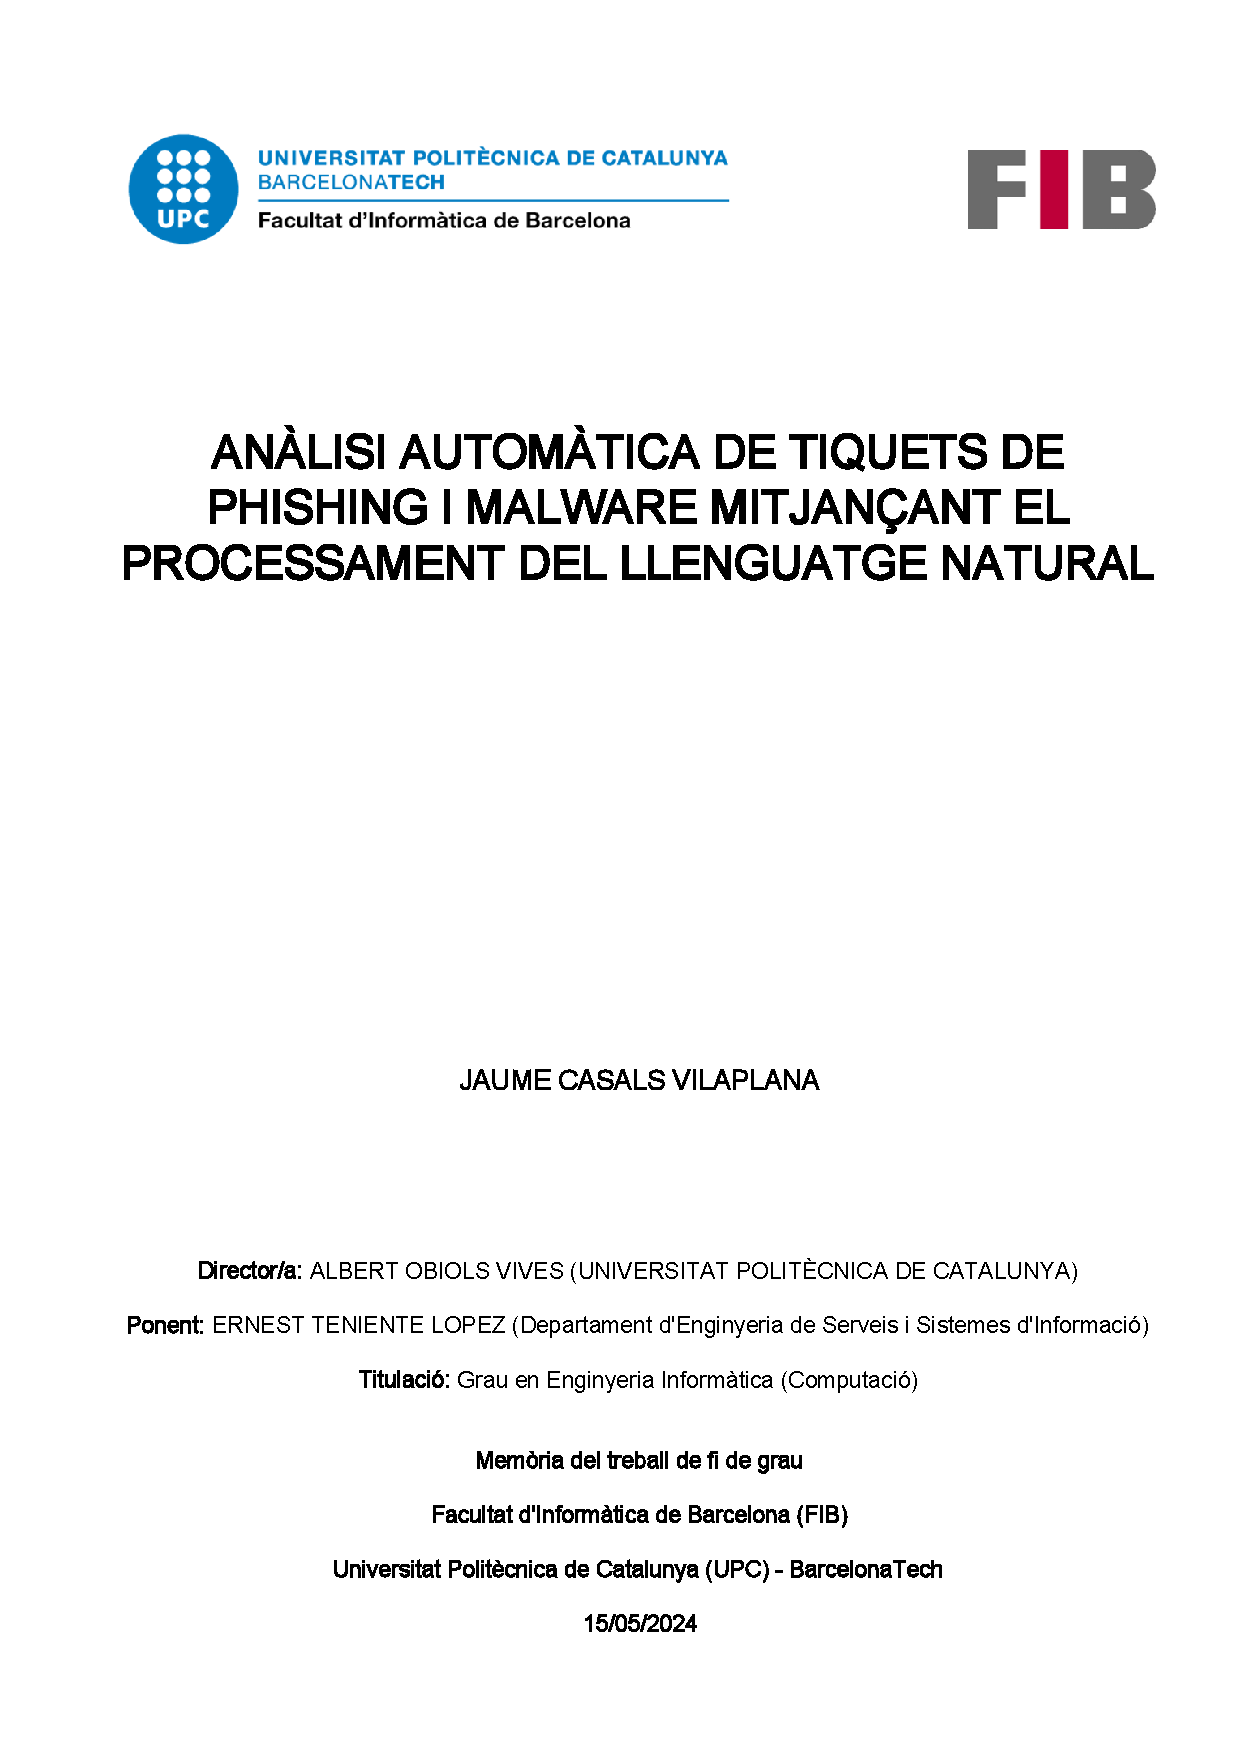
\includepdf[pages=-]{portada.pdf}

\begin{comment}
\begin{titlepage}
    \centering
    
\includegraphics[width=0.9\textwidth]{logo-upc-fib.png}
    \par\vspace{0.5cm}
    
    {\scshape\Large Grau en Enginyeria Informàtica\par}
    {\scshape\large Especialitat en Computació\par}
    
    \vspace{4.1cm}
    
    {\scshape\huge\bfseries Anàlisi automàtica de tiquets de phishing i malware mitjançant el processament del llenguatge natural
    }
    
    \vspace{2cm}
    
    {\Large\itshape Jaume Casals Vilaplana\par}
    
    \vfill
    
    Director: Ernest Teniente López\par
    Ponent: Albert Obiols Vives\par
    Tutor de GEP: Carolina Maria Consolación Segura\par
    \vspace{1.5cm}
    
\includegraphics[width=0.4\textwidth]{logo-inlab.png}
    \vspace{0.5cm}
    {\par\large\today\par}
    
\end{titlepage}
\end{comment}
\clearpage

\pagenumbering{gobble} % Avoid page numbering
\chapter*{\centering Resum}
Aquest informe descriu un projecte desenvolupat per millorar la gestió d'incidents en una empresa de ciberseguretat mitjançant l'ús d'un model de Processament del Llenguatge Natural (NLP). L'objectiu principal és l'extracció de certs camps dels tiquets d'incidents, completant un sistema automàtic per la millor experiència d'usuari. El projecte aborda els reptes del volum creixent i complexitat dels incidents de ciberseguretat, utilitzant un model de NLP que ha estat perfeccionat per comprendre els matisos lingüístics i contextuals dels textos d'entrada, tenint en compte les limitacions tècniques presents. La solució implementada inclou un procés complet de l'extracció de la informació, que inclou la recuperació dels tiquets, les tècniques de preprocessament adaptades i l'extracció de característiques clau. S'emfatitza la seguretat i la confidencialitat de la informació delicada durant tot el procés. La implementació d'aquest sistema no només millora l'eficiència operativa, sinó que també contribueix a millorar la resposta a les amenaces cibernètiques en constant evolució i enforteix la postura de ciberseguretat de l'empresa i la comunitat en general.

\chapter*{\centering Resumen}
Este informe describe un proyecto desarrollado para mejorar la gestión de incidentes en una empresa de ciberseguridad mediante el uso de un modelo de Procesamiento del Lenguaje Natural (NLP). El objetivo principal es la extracción de ciertos campos de los tiques de incidentes, completando un sistema automático para la mejor experiencia de usuario. El proyecto aborda los retos del creciente volumen y complejidad de los incidentes de ciberseguridad, utilizando un modelo de NLP que ha sido perfeccionado para comprender los matices lingüísticos y contextuales de los textos de entrada, teniendo en cuenta las limitaciones técnicas presentes. La solución implementada incluye un proceso completo de la extracción de la información, que incluye la recuperación de los tiques, las técnicas de preprocesamiento adaptadas y la extracción de características clave. Se enfatiza la seguridad y confidencialidad de la información delicada durante todo el proceso. La implementación de este sistema no solo mejora la eficiencia operativa, sino que también contribuye a mejorar la respuesta a las amenazas cibernéticas en constante evolución y fortalece la postura de ciberseguridad de la empresa y la comunidad en general.

\chapter*{\centering Abstract}
This report describes a project developed to improve incident management in a cybersecurity company by using a Natural Language Processing (NLP) model. The main objective is the extraction of certain fields from incident tickets, completing an automatic system for the best user experience. The project addresses the challenges of the increasing volume and complexity of cybersecurity incidents, using an NLP model that has been refined to understand the linguistic and contextual nuances of the input texts, taking into account the technical limitations present. The implemented solution includes a complete process of information extraction, including ticket retrieval, adapted preprocessing techniques and the extraction of certain fields. The security and confidentiality of sensitive information are emphasized throughout the process. The implementation of this system not only improves operational efficiency, but also contributes to an improved response to evolving cyber threats and strengthens the cybersecurity posture of the company and the community as a whole.

\clearpage

\pagenumbering{gobble} % Avoid page numbering

\selectlanguage{catalan}                        % Idioma índex
\tableofcontents
\listoftables
\listoffigures
\clearpage

\pagenumbering{arabic}

%% Index esperat:
\begin{comment}
            ANÀLISI DE TIQUETS D'INCIDÈNCIES MITJANÇANT PROCESSAMENT DEL LLENGUATGE NATURAL (NLP)
1 Contextualització i abast
    1.1 Contextualització 
        1.1.1 Context 
        1.1.2 Problema a resoldre 
        1.1.3 Actors implicats 
        [?] 1.1.4 Justificació
        1.1.5 Lleis i regulacions 
    1.2 Abast 
        1.2.1 Objectius 
        1.2.2 Requisits funcionals 
        1.2.3 Requisits no funcionals 
        1.2.4 Obstacles i riscos potencials 
    1.3 Metodologia i rigor 
        1.3.1 Metodologia 
        1.3.2 Eines 
2 Exploració teòrica
    2.1 Conceptes generals
        2.1.1 Anàlisi d'un tiquet
        2.1. etc.
    2.2 Aprenentatge autònom 
        2.2.1 Models en general
        2.2.2 Models NLP
    2.3 Estat de l'art
        2.3.1 Aplicacions comercials
        2.3.2 Propostes descartades
        2.3.3 Comprovació models disponibles
            Models destacats
        2.3.4 Justificació de la tria
3 Desenvolupament del sistema
    3.1 Arquitectura teòrica del sistema (pipeline)
    3.2 Creació dataset teòric
    [?] 3.3 Creació de tests
    3.4 Finetune teòric
    3.5 Dataset i finetune amb dades reals
        3.5.1 Estadístiques descriptives
        3.5.2 Tendències i patrons
        3.5.3 Problemes i incidències comunes
        3.5.4 Anomalies i valors atípics
    3.6 Desplegament API
4 Avaluació amb resultats reals
    4.1 Eficàcia de la solució i anàlisi de resultats
5 Planificació temporal
    5.1 Descripció de les tasques 
        5.1.1 Gestió de Projecte [GP] (180 hores) 
        5.1.2 Treball Previ [TP] (80 hores) 
        5.1.3 Desenvolupament [D] (340 hores) 
    5.2 Recursos 
        5.2.1 Recursos humans 
        5.2.2 Recursos materials 
    5.3 Taula de tasques 
    5.4 Diagrama de Gantt 
    5.5 Gestió del risc 
6 Gestió Econòmica
    6.1 Costos de personal i activitat 
    6.2 Costos genèrics 
        6.2.1 Amortitzacions 
        6.2.2 Consum elèctric 
        6.2.3 Connexió internet 
        6.2.4 Espai d'oficina 
        6.2.5 Total costos genèrics 
    6.3 Contingències 
    6.4 Imprevistos 
    6.5 Cost total del projecte 
    6.6 Control de gestió 
    [?] 6.7 Valoració econòmica final
7 Sostenibilitat
    7.1 Autoavaluació 
    7.2 Dimensió econòmica 
    7.3 Dimensió ambiental 
    7.4 Dimensió social 
8 Integració del coneixement
    8.1 Competències tècniques del projecte
    8.2 coneixement de les assignatures
9 Conclusions 
    9.1 Assoliment dels objectius
        9.1.1 Estudi de l'estat de l'art
        9.1.2 Sistema d'extracció d'informació
        9.1.3 Implementació del pipeline
        9.1.4 Desplegament API
    9.2 Treball futur
    9.3 Conclusions personals
Apèndixs
    A. Exemples de tiquets d'incidències
\end{comment}

\clearpage

\import{./}{10-contextualitzacio_i_abast/10-main}
\clearpage

\import{./}{20-exploracio_teorica/20-main}
\clearpage

\import{./}{30-desenvolupament/30-main}
\clearpage

\import{./}{40-avaluacio/40-main}
\clearpage

\import{./}{50-planificacio_temporal/50-main}
\clearpage

\import{./}{60-gestio_economica/60-main}
\clearpage

\import{./}{70-sostenibilitat/70-main}
\clearpage

\import{./}{80-coneixement/80-main}
\clearpage

\import{./}{90-conclusions/90-main}
\clearpage

\import{./}{100-apendix/100-main}
\clearpage

\appendix

\printbibliography[title={Referències}]

\afterpage{\null\newpage}

\end{document}

ANÀLISI AUTOMÀTICA DE TIQUETS DE PHISHING I MALWARE MITJANÇANT EL PROCESSAMENT DEL LLENGUATGE NATURAL
1 Contextualització i abast
    1.1 Contextualització 
        1.1.1 Context 
        1.1.2 Problema a resoldre 
        1.1.3 Actors implicats 
        [?] 1.1.4 Justificació
        1.1.5 Lleis i regulacions 
    1.2 Abast 
        1.2.1 Objectius 
        1.2.2 Requisits funcionals 
        1.2.3 Requisits no funcionals 
        1.2.4 Obstacles i riscos potencials 
    1.3 Metodologia i rigor 
        1.3.1 Metodologia 
        1.3.2 Eines 
2 Exploració teòrica
    2.1 Conceptes generals
        2.1.1 Anàlisi d'un tiquet
        2.1.2 Phishing
        2.1.2 Malware
        2.1.2 Dataset
    2.2 Aprenentatge autònom 
        2.2.1 Models en general
        2.2.2 Models NLP
    2.3 Estat de l'art
        2.3.1 Aplicacions comercials
        2.3.2 Propostes descartades
        2.3.3 Comprovació models disponibles
        2.3.4 Models destacats
        2.3.5 Justificació de la tria
3 Desenvolupament del sistema
    3.1 Arquitectura del sistema (pipeline)
    3.2 Creació dataset sintètic
    [?] 3.3 Creació de tests
    3.4 Fine-tune sintètic
    3.5 Dataset i fine-tune amb dades reals
        3.5.1 Estadístiques descriptives
        3.5.2 Tendències i patrons
        3.5.3 Problemes i incidències comunes
        3.5.4 Anomalies i valors atípics
    3.6 Desplegament API
4 Avaluació amb resultats reals
    4.1 Eficàcia de la solució i anàlisi de resultats
5 Planificació temporal
    5.1 Descripció de les tasques 
        5.1.1 Gestió de Projecte [GP] (180 hores) 
        5.1.2 Treball Previ [TP] (80 hores) 
        5.1.3 Desenvolupament [D] (340 hores) 
    5.2 Recursos 
        5.2.1 Recursos humans 
        5.2.2 Recursos materials 
    5.3 Taula de tasques 
    5.4 Diagrama de Gantt 
    5.5 Gestió del risc 
6 Gestió Econòmica
    6.1 Costos de personal i activitat 
    6.2 Costos genèrics 
        6.2.1 Amortitzacions 
        6.2.2 Consum elèctric 
        6.2.3 Connexió internet 
        6.2.4 Espai d'oficina 
        6.2.5 Total costos genèrics 
    6.3 Contingències 
    6.4 Imprevistos 
    6.5 Cost total del projecte 
    6.6 Control de gestió 
    [?] 6.7 Valoració econòmica final
7 Sostenibilitat
    7.1 Autoavaluació 
    7.2 Dimensió econòmica 
    7.3 Dimensió ambiental 
    7.4 Dimensió social 
8 Integració del coneixement
    8.1 Competències tècniques del projecte
    8.2 coneixement de les assignatures
9 Conclusions 
    9.1 Assoliment dels objectius
        9.1.1 Estudi de l'estat de l'art
        9.1.2 Sistema d'extracció d'informació
        9.1.3 Implementació del pipeline
        9.1.4 Desplegament API
    9.2 Treball futur
    9.3 Conclusions personals
Apèndixs
    A. Exemples de tiquets d'incidències
